%!TEX root = ../thesis.tex

\chapter{Background}
\label{cha:background}

\section{Section A}
\label{sec:section_a}
This is how to use section, subsections, and subsubsections. Don't forget to use labels right from the beginning, otherwise you'll have to work a lot if the text is already written. Don't be lazy, it'll pay off in the long run.
\subsection{Subsection A1}
\label{sub:subsection_a1}
Blah blah.
\subsubsection{Subsection A1i}
\label{ssub:subsection_a1i}
Blah blah.
% subsubsection subsection_a1i (end)

% subsection subsection_a1 (end)

% section section_a (end)

\section{Including Images}
\label{sec:images}

Lorem ipsum dolor sit amet, consectetur adipisicing elit, sed do eiusmod
tempor incididunt ut labore et dolore magna aliqua. Ut enim ad minim veniam,
quis nostrud exercitation ullamco laboris nisi ut aliquip ex ea commodo
consequat. Duis aute irure dolor in reprehenderit in voluptate velit esse
cillum dolore eu fugiat nulla pariatur. Excepteur sint occaecat cupidatat non
proident, sunt in culpa qui officia deserunt mollit anim id est laborum in Figure \ref{fig:femto_over_DSL_deployment}.

\begin{figure}[h!]
\centering
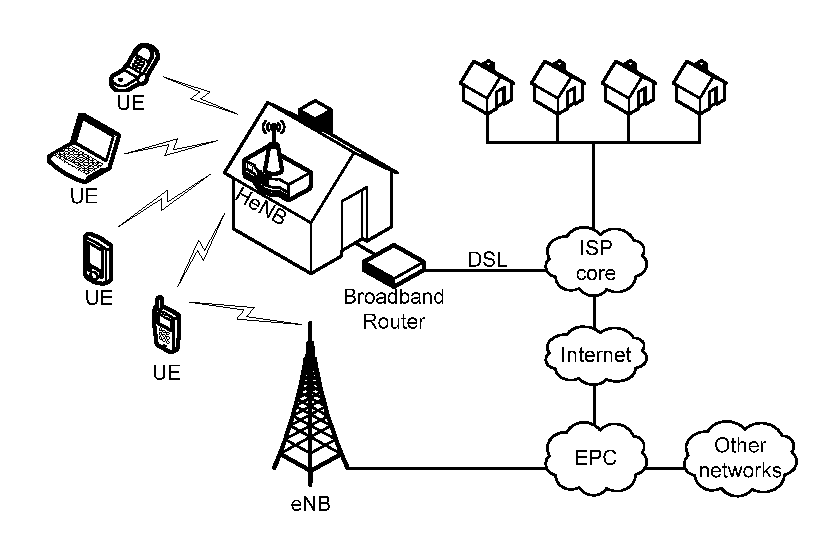
\includegraphics[width=2.25in, angle=123]{typical_femtocell_deployment.eps}
\caption{Typical deployment for LTE Femtocells with DSL backhaul}
\label{fig:femto_over_DSL_deployment}
\end{figure}

Lorem ipsum dolor sit amet, consectetur adipisicing elit, sed do eiusmod
tempor incididunt ut labore et dolore magna aliqua. Ut enim ad minim veniam,
quis nostrud exercitation ullamco laboris nisi ut aliquip ex ea commodo
consequat. Duis aute irure dolor in reprehenderit in voluptate velit esse
cillum dolore eu fugiat nulla pariatur. Excepteur sint occaecat cupidatat non
proident, sunt in culpa qui officia deserunt mollit anim id est laborum.

Lorem ipsum dolor sit amet, consectetur adipisicing elit, sed do eiusmod
tempor incididunt ut labore et dolore magna aliqua. Ut enim ad minim veniam,
quis nostrud exercitation ullamco laboris nisi ut aliquip ex ea commodo
consequat. Duis aute irure dolor in reprehenderit in voluptate velit esse
cillum dolore eu fugiat nulla pariatur. Excepteur sint occaecat cupidatat non
proident, sunt in culpa qui officia deserunt mollit anim id est laborum.
% section images (end)

\section{Tables}
\label{sec:tables}

Lorem ipsum dolor sit amet, consectetur adipisicing elit, sed do eiusmod
tempor incididunt ut labore et dolore magna aliqua. Ut enim ad minim veniam,
quis nostrud exercitation ullamco laboris nisi ut aliquip ex ea commodo
consequat. Duis aute irure dolor in reprehenderit in voluptate velit esse
cillum dolore eu fugiat nulla pariatur. Excepteur sint occaecat cupidatat non
proident, sunt in culpa qui officia deserunt mollit anim id est laborum in Table \ref{table_label}

\begin{table}[h!]
    \centering
    \begin{tabular}{ccccccc}
    % \cline{1-3}
    \toprule
     & \multicolumn{2}{c}{\bf{$iMOS$}} & \multicolumn{2}{c}{\bf{$\mu(iMOS)$}} & \multicolumn{2}{c}{\bf{$\sigma(iMOS)$}}\\
    \cmidrule(r){2-3} \cmidrule(r){4-5} \cmidrule(r){6-7}
    \bf{Call} & \bf{DL} & \bf{UL} & \bf{DL} & \bf{UL} & \bf{DL} & \bf{UL}\\ 
    \cmidrule(r){1-1} \cmidrule(r){2-7}
    % \midrule
    $call_1$ & 3.90, 3.90, ..., 3.80 & 3.73, 3.81, ..., 3.69 & 3.88 & 3.78 & 0.4 & 0.6 \\ 
    $call_2$ & 3.82, 3.80, ..., 3.80 & 3.70, 3.73, ..., 3.75 & 3.81 & 3.71 & 0.2 & 0.3 \\
    ... & ... & ... & ... & ... & ... & ... \\ 
    $call_M$ & 3.85, 3.80, ..., 3.75 & 3.75, 3.70, ..., 3.65 & 3.80 & 3.70 & 0.5 & 0.5 \\
    \midrule
    
    & \multicolumn{2}{r}{\textcolor{blue}{$\mu(\mu(iMOS))$}} & \textcolor{blue}{3.74} & \textcolor{blue}{3.84} & & \\
    
    & \multicolumn{2}{r}{\textcolor{blue}{$\sigma(\mu(iMOS))$}} & \textcolor{blue}{0.04} & \textcolor{blue}{0.06} & &  \\
    
    & \multicolumn{2}{r}{\textcolor{blue}{$\mu(\sigma(iMOS))$}} &  & & \textcolor{blue}{0.33} & \textcolor{blue}{0.53} \\
    
    \bottomrule
    \end{tabular}
    \caption{Obtaining the Mean ($\mu$) and Standard Deviation ($\sigma$) of iMOS}
    \label{table_label}
  \end{table}

% section tables (end)

\section{Equations}
\label{sec:equations}
Lorem ipsum dolor sit amet, consectetur adipisicing elit, sed do eiusmod
tempor incididunt ut labore et dolore magna aliqua. Ut enim ad minim veniam,
quis nostrud exercitation ullamco laboris nisi ut aliquip ex ea commodo
consequat. Duis aute irure dolor in reprehenderit in voluptate velit esse
cillum dolore eu fugiat nulla pariatur. Excepteur sint occaecat cupidatat non
proident, sunt in culpa qui officia deserunt mollit anim id est laborum in Equation (\ref{eq:heavyside_function}).

\begin{equation}\label{eq:heavyside_function}
H(x) = 
\begin{cases}
0 &\text{$if$ $x < 0,$ $else$}\\
1 &\text{$for$ $x \geq 0$}
\end{cases}
\end{equation}

Lorem ipsum dolor sit amet, consectetur adipisicing elit, sed do eiusmod
tempor incididunt ut labore et dolore magna aliqua. Ut enim ad minim veniam,
quis nostrud exercitation ullamco laboris nisi ut aliquip ex ea commodo
consequat. Duis aute irure dolor in reprehenderit in voluptate velit esse
cillum dolore eu fugiat nulla pariatur. Excepteur sint occaecat cupidatat non
proident, sunt in culpa qui officia deserunt mollit anim id est laborum.

% section equations (end)


\section{Algorithms}
\label{sec:algorithms}
Lorem ipsum dolor sit amet, consectetur adipisicing elit, sed do eiusmod
tempor incididunt ut labore et dolore magna aliqua. Ut enim ad minim veniam,
quis nostrud exercitation ullamco laboris nisi ut aliquip ex ea commodo
consequat. Duis aute irure dolor in reprehenderit in voluptate velit esse
cillum dolore eu fugiat nulla pariatur. Excepteur sint occaecat cupidatat non
proident, sunt in culpa qui officia deserunt mollit anim id est laborum in Algorithm \ref{algo:my_algo}.

\begin{algorithm}[h!]
 \SetKwInOut{Input}{input}
 \SetKwInOut{Output}{output}

\Input{x, y}
\Output{z}
\BlankLine
\eIf{$x>y$}{
	do this\;
   }{
      \For{$i \leftarrow 1$ \KwTo $10$}{
        \eIf{condition}{
          \If{another condition}{
          do something\;
          }
          something else\;
        }{
        whatever; \emph{// your comment}
        }
      }
}
Done

\caption{How to ...}
\label{algo:my_algo}
\end{algorithm}

% section algorithms (end)

\section{Citations}
\label{sec:citations}
\citeauthor{einstein1905electrodynamics} in \cite{einstein1905electrodynamics} have done this and that.
% section citations (end)

\section{Acronyms}
\label{sec:acronyms}
\ac{VoIP} is bla bla. \ac{WMN} is that. If you want it full again: \acf{VoIP}. If you want only its extended text, then use \acl{WMN}. If you want plural use: for acronym \acp{WMN}, and full \& long version \aclp{WMN}. Take care, some plurals in English are special.
% section acronyms (end)

\section{To dos}
\label{sec:to_dos}
In case you want to do something later and want to make sure not to forget, leave a marker on the margin, like this \todo{Dont't forget this.}. If you enable the list of todos in the main file, i.e. thesis.tex via the \emph{listoftodos} command, then you'll have them all centralized on one page. So you know the scale of what you have to do!
% section to_dos (end)

% chapter background (end)